\documentclass{standalone}
\usepackage{tikz}
\usetikzlibrary{patterns, positioning}
\usepackage[sfdefault]{ClearSans} %% option 'sfdefault' activates Clear Sans as the default text font
\usepackage[T1]{fontenc}

\begin{document}
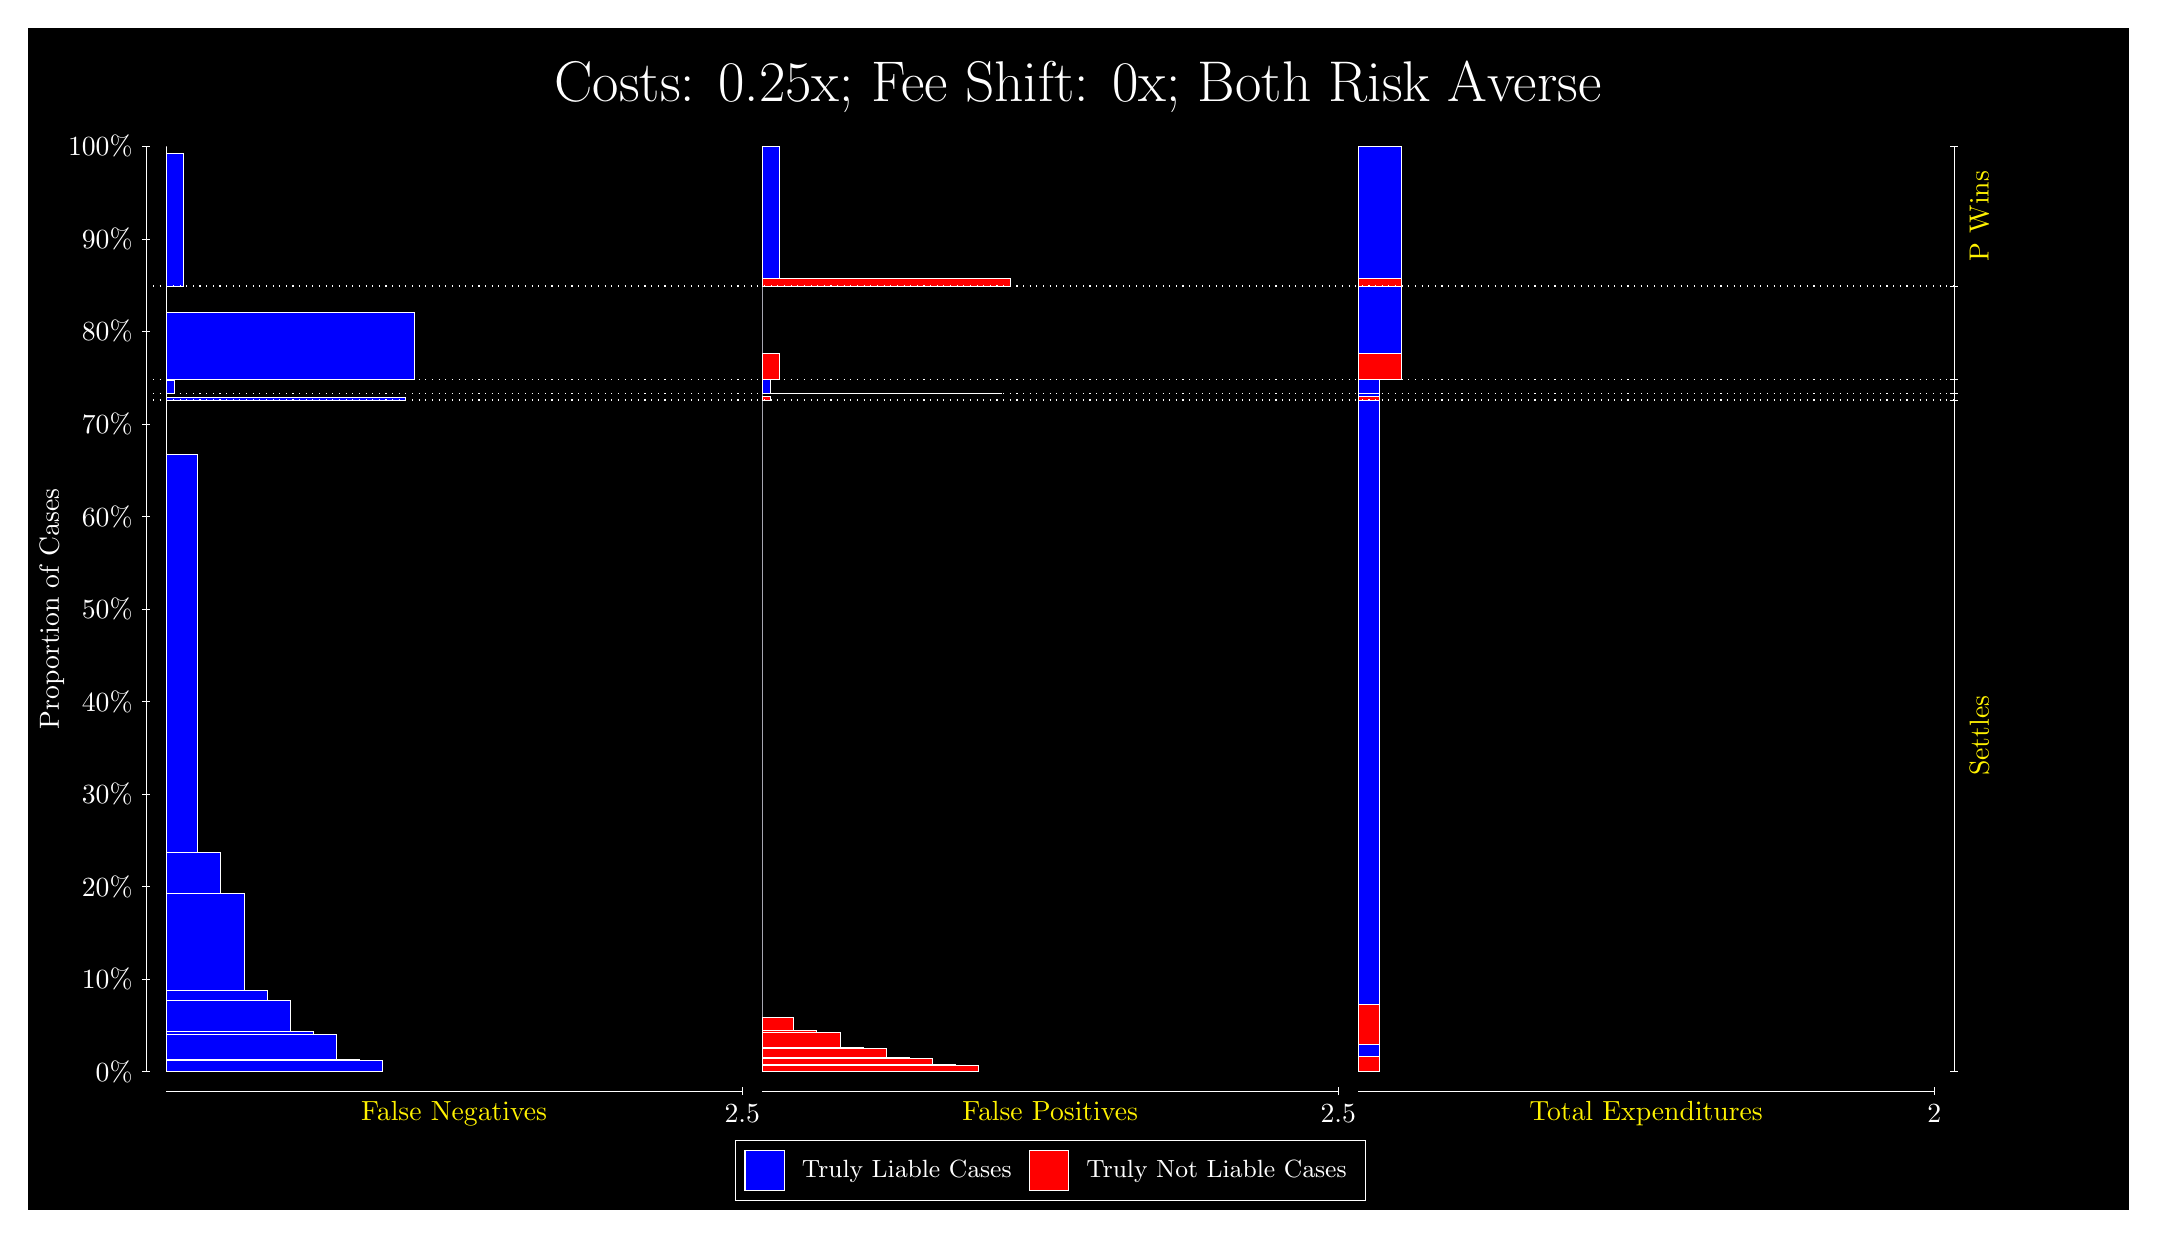
\begin{tikzpicture}
\draw[fill=black] (0,0) rectangle (26.667,15);
\draw[text=white] (0,13.5) rectangle (26.667,15) node[midway] {\huge Costs: 0.25x; Fee Shift: 0x; Both Risk Averse};
\draw[white, very thin] (1.5,1.75) -- (1.5,13.5);
\node[rotate=90, text=white, anchor=center] at (0.3, 7.625) {Proportion of Cases};
\draw[white, very thin] (1.45,1.75) -- (1.55,1.75);
\node[text=white, anchor=east] at (1.45, 1.75) {0\%};
\draw[white, very thin] (1.45,2.925) -- (1.55,2.925);
\node[text=white, anchor=east] at (1.45, 2.925) {10\%};
\draw[white, very thin] (1.45,4.1) -- (1.55,4.1);
\node[text=white, anchor=east] at (1.45, 4.1) {20\%};
\draw[white, very thin] (1.45,5.275) -- (1.55,5.275);
\node[text=white, anchor=east] at (1.45, 5.275) {30\%};
\draw[white, very thin] (1.45,6.45) -- (1.55,6.45);
\node[text=white, anchor=east] at (1.45, 6.45) {40\%};
\draw[white, very thin] (1.45,7.625) -- (1.55,7.625);
\node[text=white, anchor=east] at (1.45, 7.625) {50\%};
\draw[white, very thin] (1.45,8.8) -- (1.55,8.8);
\node[text=white, anchor=east] at (1.45, 8.8) {60\%};
\draw[white, very thin] (1.45,9.975) -- (1.55,9.975);
\node[text=white, anchor=east] at (1.45, 9.975) {70\%};
\draw[white, very thin] (1.45,11.15) -- (1.55,11.15);
\node[text=white, anchor=east] at (1.45, 11.15) {80\%};
\draw[white, very thin] (1.45,12.325) -- (1.55,12.325);
\node[text=white, anchor=east] at (1.45, 12.325) {90\%};
\draw[white, very thin] (1.45,13.5) -- (1.55,13.5);
\node[text=white, anchor=east] at (1.45, 13.5) {100\%};

\draw[white, very thin] (24.457,1.75) -- (24.457,13.5);
\draw[white, very thin] (24.407,1.75) -- (24.507,1.75);
\node[anchor=west] at (24.407, 1.75) {};
\draw[white, very thin] (24.407,10.279) -- (24.507,10.279);
\node[anchor=west] at (24.407, 10.279) {};
\draw[white, very thin] (24.407,10.362) -- (24.507,10.362);
\node[anchor=west] at (24.407, 10.362) {};
\draw[white, very thin] (24.407,10.537) -- (24.507,10.537);
\node[anchor=west] at (24.407, 10.537) {};
\draw[white, very thin] (24.407,11.726) -- (24.507,11.726);
\node[anchor=west] at (24.407, 11.726) {};
\draw[white, very thin] (24.407,13.5) -- (24.507,13.5);
\node[anchor=west] at (24.407, 13.5) {};

\draw[white, very thin, fill=blue] (1.75,1.75) rectangle (4.4946,1.8871);
\draw[white, very thin, fill=blue] (1.75,1.8871) rectangle (4.2018,1.9068);
\draw[white, very thin, fill=blue] (1.75,1.9068) rectangle (3.9091,2.224);
\draw[white, very thin, fill=blue] (1.75,2.224) rectangle (3.6163,2.2671);
\draw[white, very thin, fill=blue] (1.75,2.2671) rectangle (3.3236,2.6496);
\draw[white, very thin, fill=blue] (1.75,2.6496) rectangle (3.0308,2.7782);
\draw[white, very thin, fill=blue] (1.75,2.7782) rectangle (2.738,4.0179);
\draw[white, very thin, fill=blue] (1.75,4.0179) rectangle (2.4453,4.5301);
\draw[white, very thin, fill=blue] (1.75,4.5301) rectangle (2.1525,9.5859);
\draw[white, very thin, fill=red] (1.75,9.5859) rectangle (1.75,10.279);
\draw[white, very thin, fill=blue] (1.75,10.279) rectangle (4.7873,10.31);
\draw[white, very thin, fill=red] (1.75,10.31) rectangle (1.75,10.362);
\draw[white, very thin, fill=blue] (1.75,10.362) rectangle (1.8598,10.535);
\draw[white, very thin, fill=red] (1.75,10.535) rectangle (1.75,10.537);
\draw[white, very thin, fill=blue] (1.75,10.537) rectangle (4.8971,11.392);
\draw[white, very thin, fill=red] (1.75,11.392) rectangle (1.75,11.726);
\draw[white, very thin, fill=blue] (1.75,11.726) rectangle (1.9696,13.406);
\draw[white, very thin, fill=red] (1.75,13.406) rectangle (1.75,13.5);
\draw[white, very thin, fill=red] (9.3189,1.75) rectangle (12.063,1.8351);
\draw[white, very thin, fill=red] (9.3189,1.8351) rectangle (11.771,1.8434);
\draw[white, very thin, fill=red] (9.3189,1.8434) rectangle (11.478,1.9205);
\draw[white, very thin, fill=red] (9.3189,1.9205) rectangle (11.185,1.9338);
\draw[white, very thin, fill=red] (9.3189,1.9338) rectangle (10.892,2.0412);
\draw[white, very thin, fill=red] (9.3189,2.0412) rectangle (10.6,2.0602);
\draw[white, very thin, fill=red] (9.3189,2.0602) rectangle (10.307,2.2502);
\draw[white, very thin, fill=red] (9.3189,2.2502) rectangle (10.014,2.2704);
\draw[white, very thin, fill=red] (9.3189,2.2704) rectangle (9.7214,2.4428);
\draw[white, very thin, fill=blue] (9.3189,2.4428) rectangle (9.3189,10.279);
\draw[white, very thin, fill=red] (9.3189,10.279) rectangle (9.4287,10.331);
\draw[white, very thin, fill=blue] (9.3189,10.331) rectangle (9.3189,10.362);
\draw[white, very thin, fill=red] (9.3189,10.362) rectangle (12.356,10.365);
\draw[white, very thin, fill=blue] (9.3189,10.365) rectangle (9.4287,10.537);
\draw[white, very thin, fill=red] (9.3189,10.537) rectangle (9.5384,10.871);
\draw[white, very thin, fill=blue] (9.3189,10.871) rectangle (9.3189,11.726);
\draw[white, very thin, fill=red] (9.3189,11.726) rectangle (12.466,11.82);
\draw[white, very thin, fill=blue] (9.3189,11.82) rectangle (9.5384,13.5);
\draw[white, very thin, fill=red] (16.888,1.75) rectangle (17.162,1.9425);
\draw[white, very thin, fill=blue] (16.888,1.9425) rectangle (17.162,2.0993);
\draw[white, very thin, fill=red] (16.888,2.0993) rectangle (17.162,2.5996);
\draw[white, very thin, fill=blue] (16.888,2.5996) rectangle (17.162,10.279);
\draw[white, very thin, fill=red] (16.888,10.279) rectangle (17.162,10.331);
\draw[white, very thin, fill=blue] (16.888,10.331) rectangle (17.162,10.362);
\draw[white, very thin, fill=red] (16.888,10.362) rectangle (17.162,10.365);
\draw[white, very thin, fill=blue] (16.888,10.365) rectangle (17.162,10.537);
\draw[white, very thin, fill=red] (16.888,10.537) rectangle (17.437,10.871);
\draw[white, very thin, fill=blue] (16.888,10.871) rectangle (17.437,11.726);
\draw[white, very thin, fill=red] (16.888,11.726) rectangle (17.437,11.82);
\draw[white, very thin, fill=blue] (16.888,11.82) rectangle (17.437,13.5);
\draw[white, dotted] (1.5,10.279) -- (24.457,10.279);
\draw[white, dotted] (1.5,10.362) -- (24.457,10.362);
\draw[white, dotted] (1.5,10.537) -- (24.457,10.537);
\draw[white, dotted] (1.5,11.726) -- (24.457,11.726);
\draw[white, very thin] (1.75,1.5) -- (9.0689,1.5);
\node[text=yellow, anchor=north] at (5.4094, 1.5) {False Negatives};
\draw[white, very thin] (9.0689,1.45) -- (9.0689,1.55);
\node[text=white, anchor=north] at (9.0689, 1.45) {2.5};

\draw[white, very thin] (9.3189,1.5) -- (16.638,1.5);
\node[text=yellow, anchor=north] at (12.978, 1.5) {False Positives};
\draw[white, very thin] (16.638,1.45) -- (16.638,1.55);
\node[text=white, anchor=north] at (16.638, 1.45) {2.5};

\draw[white, very thin] (16.888,1.5) -- (24.207,1.5);
\node[text=yellow, anchor=north] at (20.547, 1.5) {Total Expenditures};
\draw[white, very thin] (24.207,1.45) -- (24.207,1.55);
\node[text=white, anchor=north] at (24.207, 1.45) {2};

\node[text=yellow, centered, rotate=90] at (24.777, 6.0143) {Settles};



\node[text=yellow, centered, rotate=90] at (24.777, 12.613) {P Wins};

\draw (12.978300999999998,1.5) node[draw=none] (baseCoordinate) {};
\begin{scope}[align=center]
        \matrix[scale=0.5, draw=white, below=0.5cm of baseCoordinate, nodes={draw}, column sep=0.1cm]{
            \node[rectangle, draw, minimum width=0.5cm, minimum height=0.5cm, fill=blue] {}; &
            \node[draw=none, font=\small, text=white] (B) {Truly Liable Cases}; &
            \node[rectangle, draw, minimum width=0.5cm, minimum height=0.5cm, fill=red] {}; &
            \node[draw=none, font=\small, text=white] (B) {Truly Not Liable Cases}; \\
            };
\end{scope}

\end{tikzpicture}
\end{document}